\documentclass{minimal}
\usepackage{pgf}
\usepackage{tikz}
\usepackage[utf8]{inputenc}
\usepackage{tikzsymbols}
\usepackage{adjustbox}
\usetikzlibrary{arrows,automata}
\usetikzlibrary{positioning}


\tikzset{
    state/.style={
           rectangle,
           rounded corners,
           draw=black, very thick,
           minimum height=2em,
           inner sep=10pt,
           text centered,
           },
}

\begin{document}

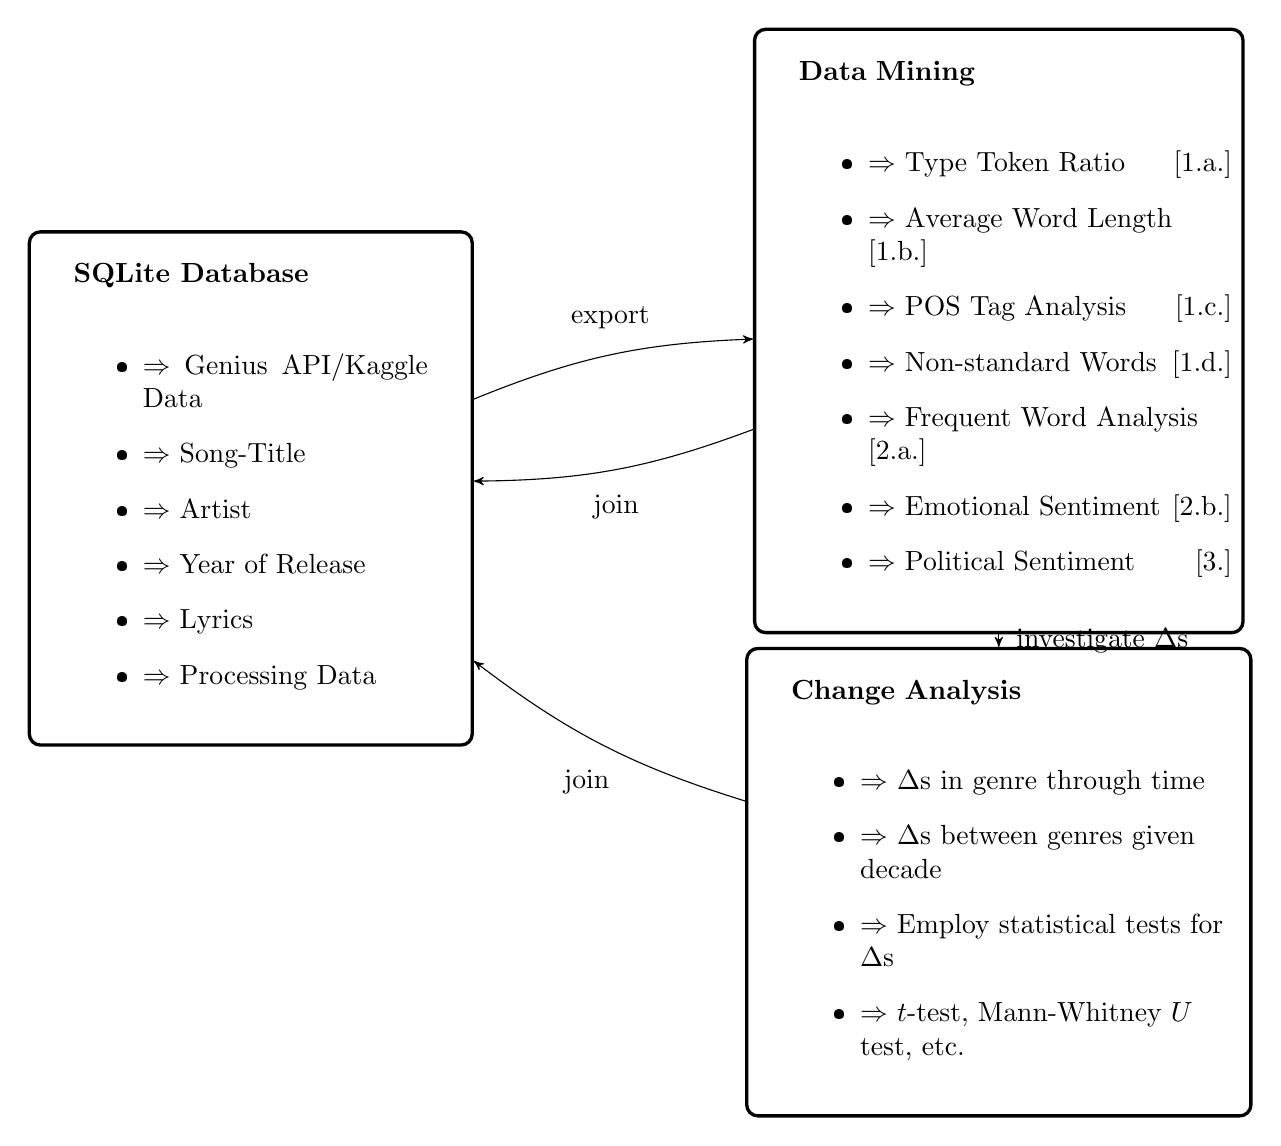
\begin{tikzpicture}[->,>=stealth']

 % Position of QUERY 
 % Use previously defined 'state' as layout (see above)
 % use tabular for content to get columns/rows
 % parbox to limit width of the listing
 \node[state] (QUERY) 
 {\begin{tabular}{l}
  \textbf{SQLite Database}\\\\
  \parbox{4.5cm}{\begin{itemize}
   \item $\Rightarrow$ Genius API/Kaggle Data
   \item $\Rightarrow$ Song-Title
   \item $\Rightarrow$ Artist
   \item $\Rightarrow$ Year of Release
   \item $\Rightarrow$ Lyrics
   \item $\Rightarrow$ Processing Data
  \end{itemize}
  }
 \end{tabular}};
  
 % State: ACK with different content
 \node[state,    	% layout (defined above)
  text width=5.5cm, 	% max text width
  yshift=2cm, 
  xshift = 3cm,		% move 2cm in y
  right of=QUERY, 	% Position is to the right of QUERY
  node distance=6.5cm, 	% distance to QUERY
  anchor=center] (P) 	% posistion relative to the center of the 'box'
 {%
 \begin{tabular}{l} 	% content
  \textbf{Data Mining}\\\\
    \parbox{5.5cm}{\begin{itemize}
    	\item $\Rightarrow$ Type Token Ratio \hfill [1.a.]
    	\item $\Rightarrow$ Average Word Length \hfill [1.b.]
    	\item $\Rightarrow$ POS Tag Analysis \hfill [1.c.]
    	\item $\Rightarrow$ Non-standard Words \hfill [1.d.]
    	\item $\Rightarrow$ Frequent Word Analysis \hfill [2.a.]
    	\item $\Rightarrow$ Emotional Sentiment \hfill [2.b.]
    	\item $\Rightarrow$ Political Sentiment \hfill [3.]
    	\end{itemize}
    }
 \end{tabular}
 };
 
 \node[state,
  below of=P,
  yshift=-6cm,
  anchor=center,
  text width=5.7cm] (C) 
 {%
 \begin{tabular}{l}
  \textbf{Change Analysis}\\\\
  \parbox{5.71cm}{\begin{itemize}
  	\item $\Rightarrow$ $\Delta$s in genre through time
  	\item $\Rightarrow$ $\Delta$s between genres given decade
  	\item $\Rightarrow$ Employ statistical tests for $\Delta$s
  	\item $\Rightarrow$ $t$-test, Mann-Whitney $U$ test, etc.
  	\end{itemize}
  }
 \end{tabular}
 };

 % draw the paths and and print some Text below/above the graph
 \path 
 (QUERY) 	edge[bend left=10]  node[anchor=south,above, yshift = 0.2cm]{export} (P)
 
 (P) 	edge[bend left=10]  node[anchor=north,below, yshift = -0.2cm]{join}
                                    node[anchor=north,below]{} (QUERY)

 (C)     	edge[bend left=10] node[anchor=south,below,xshift = -0.2cm, yshift = -0.2cm]{join} (QUERY)
 (P)  	edge                node[anchor=left,right, xshift = 0.1cm]{investigate $\Delta$s} (C);

\end{tikzpicture}
\end{document}
